\chapter*{Исполнитель Черепаха}
\addtocounter{chapter}{1}

\section{Общие сведения}

\subsection{Цель разработки и содержимое поставки}

Цель разработки --- создание исполнителя Черепаха в соответствии с учебником «Инфор\-ма\-тика-6». Настоящая поставка содержит прототип исполнителя, работающего в автономном режиме (см. ниже). Взаимодействие исполнителя с системой КуМир в настоящее время отлаживается.
 
\subsection{Платформа разработки}

Как и система Кумир 1.7.0, исполнитель Черепаха разрабатывается с помощью библиотеки классов Qt~4 и, таким образом, является кросс-платформенной разработкой. В настоящее время созданы версии для Windows и Linux. 

\section{Описание работы исполнителя}

\subsection{Окна}

При запуске исполнителя создаются два окна:
\begin{itemize}
\item окно черепахи;
\item окно пульта.
\end{itemize}

Окно пульта является основным. При попытке его закрыть будкт закрыто и окно черепахи.


	
Окна пульта и черепахи можно передвигать по экрану, сворачивать и разворачивать обычным образом. Окно черепахи можно зафиксировать поверх других окон, для этого справа на заголовке имеется кнопка.

\emph{Ограничение:} размеры окон менять нельзя.

\subsection{Окно черепахи}

Окно черепахи – квадратное (см.~\ref{tortWindow}). Оно содержит желтое поле («арену, посыпанную песком»), окруженную голубой полосой («ров с водой»).

При передвижениях черепахи конец хвоста, которым черепаха рисует, не должен попадать в воду; при попытке сделать это, исполнитель выдает отказ. Сама черепаха (ее тело, голова и т.п.) может оказаться «в воде» и даже за пределами окна («под забором»). 

В соответствии с учебником, черепаха рисует кончиком хвоста (а не серединой живота, как в большинстве реализаций). Поворот черепахи происходит относительно конца хвоста. 

\begin{figure}[h]
	\begin{center}
		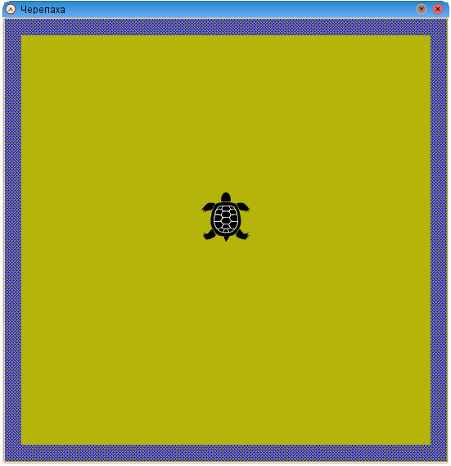
\includegraphics[scale=0.5]{tortwindow.png}
	\end{center}
	\caption{Окно Черепахи}
\label{tortWindow}
\end{figure}

Размер стороны арены --- 500 пикселей. Единица перемещения черепахи соответствует одному пикселю.

При запуске исполнителя арена пуста. Черепаха находится в центре, хост опущен. Такое состояние арены будем называть начальным.
Тело черепахи можно скрыть кликнув по полю.

\subsection{Окно пульта}

Окно пульта (см.~\ref{tortPult}) содержит:
\begin{figure}[h]
	\begin{center}
		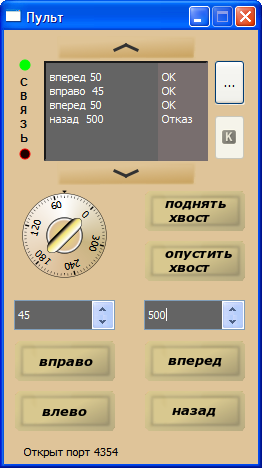
\includegraphics[scale=0.5]{tortpult.png}
	\end{center}
	\caption{Пульт управления Черепахой}
\label{tortPult}
\end{figure}

\begin{itemize}
\item поле протоколирования команд (бесконечное вниз) и кнопки прокрутки протокола (сверху и снизу от поля);
\item кнопку сброса (справа от протокола вверху); при нажатии этой кнопки арена сбрасывается в начальное положение, а поле протокола очищается;
\item кнопку передачи протокола в КуМир (справа от протокола внизу); по нажатию этой кнопки содержимое команд протокола вставляется в программу в окне редактирования системы КуМир; 
\item шесть кнопок для передачи команд черепахе («вперед», назад», «вправо», «влево», «поднять хвост», «опустить хвост»);
\item поля задания числовых параметров команд (ввод дробных значений и целых значений вне диапазона [0, 500] блокирован);
\item «циферблат» для задания и представления углов.
\end{itemize}


\subsection{Команды черепахи}
При работе под управлением КуМира Черепаха понимает следующие команды:
\begin{itemize}
\item поднять хвост 
\item опустить хвост
\item вперед (\textbf{вещ}) 
\item назад (\textbf{вещ})
\end{itemize}